% ***********************************************************
% ********* ALLISON HUME HEADER ********************
% ***********************************************************
% Version 2
\documentclass[letterpaper,10pt]{article}
\usepackage{amsmath} % AMS Math Package
\usepackage{amsthm} % Theorem Formatting
\usepackage{amssymb}	% Math symbols such as \mathbb
\usepackage{graphicx} % Allows for eps images
\usepackage{multicol} % Allows for multiple columns
\usepackage{epstopdf}
\usepackage{gensymb}
\usepackage{subfigure}
\usepackage{hyperref}
\usepackage{lscape}
\usepackage{lipsum}
\usepackage{lmodern}
\usepackage{microtype}
\usepackage[paperwidth=8.5in, paperheight=11in, margin=0.75in, bottom=0.75in]{geometry}
%\usepackage[dvips,letterpaper,margin=0.1in,bottom=0.75in]{geometry}
 % Sets margins and page size
\makeatletter % Need for anything that contains an @ command 
\makeatother % End of region containing @ commands
\renewcommand{\labelenumi}{(\alph{enumi})} % Use letters for enumerate
% \DeclareMathOperator{\Sample}{Sample}
\let\vaccent=\v % rename builtin command \v{} to \vaccent{}
\renewcommand{\v}[1]{\ensuremath{\mathbf{#1}}} % for vectors

\newcommand{\makeabs}[1]{\begin{quotation} \small #1 \end{quotation} }%make abstract
\newcommand{\tab}{\hspace{1.5mm}} %create a tab
\newcommand{\newsec}[3]{\vspace{#1} \begin{center} \textbf{#2} \vspace{#3} \end{center}}
\newcommand{\newsubsec}[3]{\vspace{#1} \large \textbf{#2} \vspace{#3} \normalsize }


\newcommand{\gv}[1]{\ensuremath{\mbox{\boldmath$ #1 $}}} 
% for vectors of Greek letters
\newcommand{\uv}[1]{\ensuremath{\mathbf{\hat{#1}}}} % for unit vector
\newcommand{\abs}[1]{\left| #1 \right|} % for absolute value
\newcommand{\avg}[1]{\left< #1 \right>} % for average
\let\underdot=\d % rename builtin command \d{} to \underdot{}
\renewcommand{\d}[2]{\frac{d #1}{d #2}} % for derivatives
\newcommand{\dd}[2]{\frac{d^2 #1}{d #2^2}} % for double derivatives
\newcommand{\pd}[2]{\frac{\partial #1}{\partial #2}} 
% for partial derivatives
\newcommand{\pdd}[2]{\frac{\partial^2 #1}{\partial #2^2}} 
% for double partial derivatives
\newcommand{\pdc}[3]{\left( \frac{\partial #1}{\partial #2}
 \right)_{#3}} % for thermodynamic partial derivatives
\newcommand{\ket}[1]{\left| #1 \right>} % for Dirac bras
\newcommand{\bra}[1]{\left< #1 \right|} % for Dirac kets
\newcommand{\braket}[2]{\left< #1 \vphantom{#2} \right|
 \left. #2 \vphantom{#1} \right>} % for Dirac brackets
\newcommand{\matrixel}[3]{\left< #1 \vphantom{#2#3} \right|
 #2 \left| #3 \vphantom{#1#2} \right>} % for Dirac matrix elements
\newcommand{\grad}[1]{\gv{\nabla} #1} % for gradient
\let\divsymb=\div % rename builtin command \div to \divsymb
\renewcommand{\div}[1]{\gv{\nabla} \cdot #1} % for divergence
\newcommand{\curl}[1]{\gv{\nabla} \times #1} % for curl
\let\baraccent=\= % rename builtin command \= to \baraccent
\renewcommand{\=}[1]{\stackrel{#1}{=}} % for putting numbers above =
\newtheorem{prop}{Proposition}
\newtheorem{thm}{Theorem}[section]
\newtheorem{lem}[thm]{Lemma}
\theoremstyle{definition}
\newtheorem{dfn}{Definition}
\theoremstyle{remark}
\newtheorem*{rmk}{Remark}

% ***********************************************************
% ********************** END HEADER *************************
% *********************************************************** % GET HEADER FROM LAST QUARTER
\begin{document}

\begin{center}

\large{\textbf{Questioning the NS-3 TCP Implementations and Suggesting Areas for Improvement}}

\vskip 5pt

Allison Hume

\end{center}

\vskip 5pt \newsec{-3mm}{Abstract}{-2mm}


\vskip 5pt \newsec{-3mm}{Introduction}{-2mm} 

\vskip 5pt \newsec{-3mm}{Results}{-2mm} 

Figure \ref{fig:WNS3} Westwood and NewReno on development simulator to compare to \cite{NS3W} Figure 10

\begin{figure}[h!]
\begin{center}
\subfigure{ 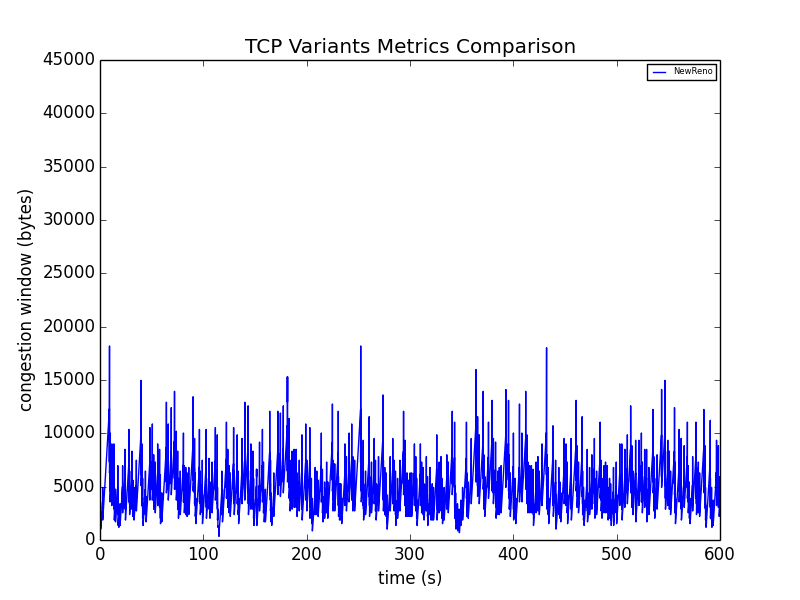
\includegraphics[trim=1cm 6.5cm 2.2cm 7.2cm, clip=true, scale=0.4]{inigo_test_results/repeatWestwoodPaper/WNS3NR.pdf}}
\subfigure{ 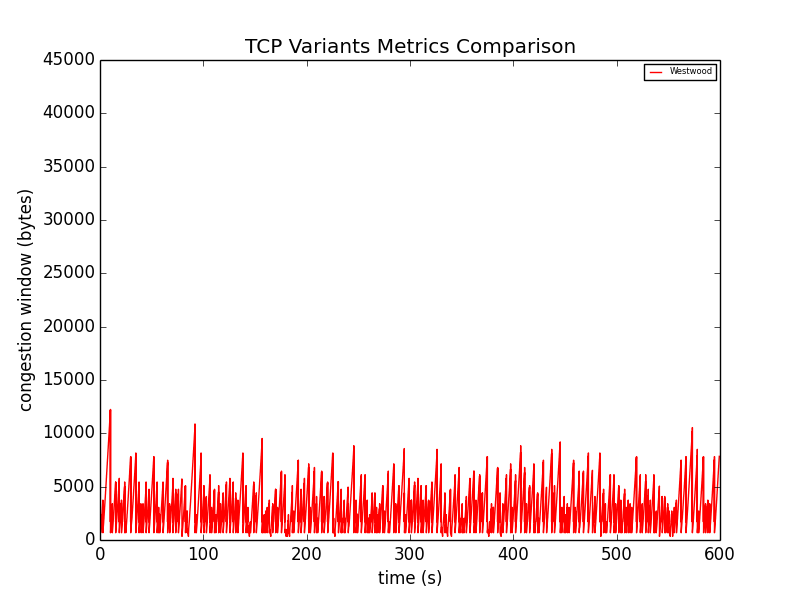
\includegraphics[trim=1cm 6.5cm 2.2cm 7.2cm, clip=true, scale=0.4]{inigo_test_results/repeatWestwoodPaper/WNS3W.pdf}}
\subfigure{ 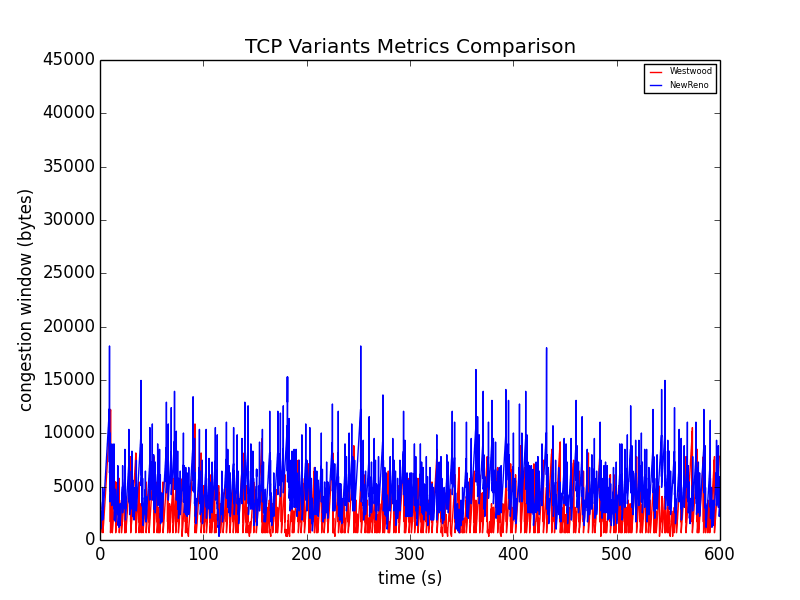
\includegraphics[trim=1cm 6.5cm 2.2cm 7.2cm, clip=true, scale=0.4]{inigo_test_results/repeatWestwoodPaper/WNS3Both.pdf}}
\end{center}
\caption{}
\label{fig:WNS3}
\end{figure}

Figure \ref{fig:WNS3Prod} Westwood and NewReno on production version 3.24 simulator to compare to \cite{NS3W} Figure 10

\begin{figure}[h!]
\begin{center}
\subfigure{ \includegraphics[trim=1cm 6.5cm 2.2cm 7.2cm, clip=true, scale=0.4]{inigo_test_results/repeatWestwoodPaper/NS3PROD/output/WNS3ProdNR.pdf}}
\subfigure{ 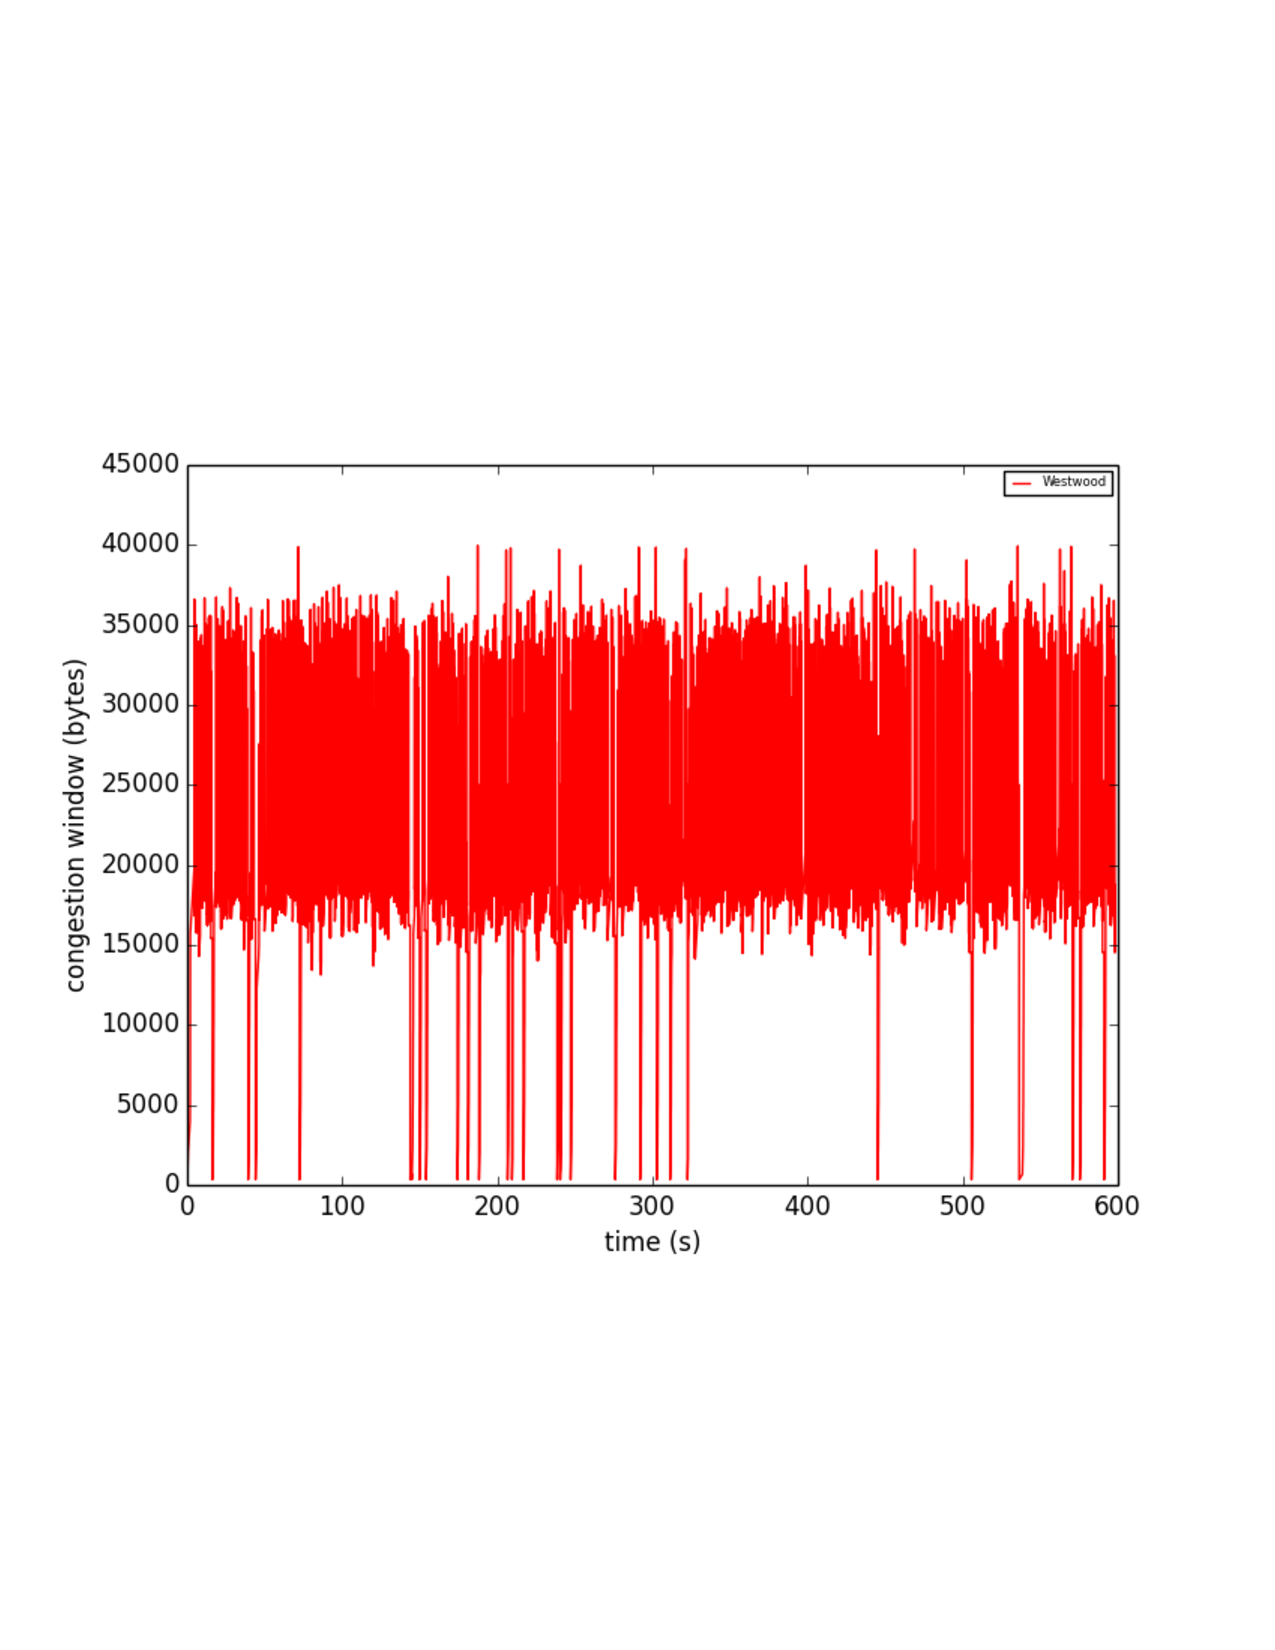
\includegraphics[trim=1cm 6.5cm 2.2cm 7.2cm, clip=true, scale=0.4]{inigo_test_results/repeatWestwoodPaper/NS3PROD/output/WNS3ProdW.pdf}}
\subfigure{ \includegraphics[trim=1cm 6.5cm 2.2cm 7.2cm, clip=true, scale=0.4]{inigo_test_results/repeatWestwoodPaper/NS3PROD/output/WNS3ProdAll.pdf}}
\end{center}
\caption{}
\label{fig:WNS3Prod}
\end{figure}

POINT: 3.24 matches decently with version from paper but dev does not match with Westwood. New Reno doesn't look bad. 

\pagebreak

Figure \ref{fig:WNS3Bug} Inigo on development simulator before and after bug fix. Same test from \cite{NS3W} Figure 10

%NEED PRE-BUG FIX PLOT AND PLOT FOR WITHOUT CLAMPS

\begin{figure}[h!]
\begin{center}
\subfigure{ \includegraphics[trim=1cm 6.5cm 2.2cm 7.2cm, clip=true, scale=0.4]{inigo_test_results/repeatWestwoodPaper/PostBF.pdf}}
\end{center}
\caption{}
\label{fig:WNS3Bug}
\end{figure}

POINT: one bug was impacting Inigo very strongly even though it wasn't super visible in New Reno or Westwood. 

Comment is quoted from \cite{RFC2582} which is specific to NewReno, not general to all TCP. 

Situation at time of comment: CA\_RECOVERY is set when there is a triple duplicate act, which triggers fast recovery. This code block is entered when a new ACK is seen and this specific case corresponds to a partial ACK. The problem was that this number was not guaranteed to be greater than zero and in extreme cases was causing overflow. Original version did not have this problem. The RFC is not completely clear on what should happen in that situation but it seems logical that that number should be positive. 

Original Code:

\begin{verbatim}

     else if (m_tcb->m_congState == TcpSocketState::CA_RECOVERY)
        {
          if (tcpHeader.GetAckNumber () < m_recover)
            {
              /* Partial ACK.
               * In case of partial ACK, retransmit the first unacknowledged
               * segment. Deflate the congestion window by the amount of new
               * data acknowledged by the Cumulative Acknowledgment field.
               * If the partial ACK acknowledges at least one SMSS of new data,
               * then add back SMSS bytes to the congestion window.
               * This artificially inflates the congestion window in order to
               * reflect the additional segment that has left the network.
               * Send a new segment if permitted by the new value of cwnd.
               * This "partial window deflation" attempts to ensure that, when
               * fast recovery eventually ends, approximately ssthresh amount
               * of data will be outstanding in the network.  Do not exit the
               * fast recovery procedure (i.e., if any duplicate ACKs subsequently
               * arrive, execute step 4 of Section 3.2 of [RFC5681]).
                */
              if (segsAcked >= 1)
                {
                  m_tcb->m_cWnd += m_tcb->m_segmentSize - bytesAcked;
                }
              else
                {
                  m_tcb->m_cWnd -= bytesAcked;
                }

              callCongestionControl = false; // No congestion control on cWnd show be invoked
              m_dupAckCount -= segsAcked;    // Update the dupAckCount
              m_txBuffer->DiscardUpTo (tcpHeader.GetAckNumber ());  //Bug 1850:  retransmit before newack
              DoRetransmit (); // Assume the next seq is lost. Retransmit lost packet

\end{verbatim}

Fixed Code:

\begin{verbatim}
              if (segsAcked >= 1)
                {
                  int diff = m_tcb->m_segmentSize - bytesAcked;
                  if (diff > 0) {
                    uint32_t cwnd = m_tcb->m_cWnd + diff;
                  }
                }
\end{verbatim}

Code in Production version of Simulator:

\begin{verbatim}
            m_tcb->m_cWnd = SafeSubtraction (m_tcb->m_cWnd, bytesAcked);
            if (segsAcked >= 1)
	    {
                m_tcb->m_cWnd += m_tcb->m_segmentSize;
             }
\end{verbatim}


Compare to \cite{NS3Val} Figure 1, which compares NewReno on ns3-3.22 to Linux.

%REDO ALL OF THIS - FIX MTU/MSS STUFF, FIGURE OUT HOW TO SET MTU ETC AND MAKE PLOT LIMITS SAME AS ORIG PAPER

\begin{figure}[h!]
\begin{center}
\subfigure{ 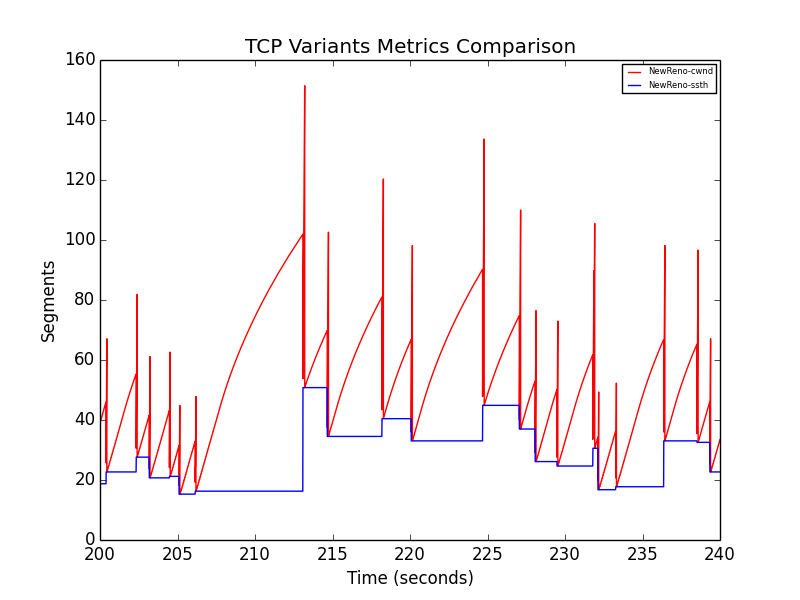
\includegraphics[trim=1cm 6.5cm 2.2cm 7.2cm, clip=true, scale=0.4]{inigo_test_results/repeatValidationPaper/ProdVersionPlot200240.pdf}}
\subfigure{ \includegraphics[trim=1cm 6.5cm 2.2cm 7.2cm, clip=true, scale=0.4]{inigo_test_results/repeatValidationPaper/NRDev.pdf}}
\end{center}
\caption{}
\label{fig:NS3Val}
\end{figure}

%\begin{table}[h!]
%\centering
%\begin{tabular}{|l|l|}
%\hline
%Experiment & Parameters \\ \hline
%\hline
%\end{tabular}
%\caption{Summary of Experiments} 
%\label{table:topos}
%\end{table}

\cite{SACK}
\cite{NS2WP}
\cite{NS2Val}
\cite{NS2Linux}

\cite{NS2TCPQ}

\cite{LinuxTCP}
\cite{RFC2582}
\cite{RFC6582}

{\small \bibliography{mybib}{}
\bibliographystyle{plain}}

\end{document}